\documentclass{report}

\usepackage{amsmath, amssymb, array, bm, enumerate, tikz, pgfplots, sfmath, multicol, hyperref, afterpage}
\pgfplotsset{compat = newest}
\usepackage[margin = 0.5in]{geometry}
\raggedright
\usepackage[scale=1.5]{ccicons}
\renewcommand{\familydefault}{\sfdefault}
\newcounter{Review}
\usetikzlibrary{fadings}
\tikzset{>=stealth}

\begin{document}

\newcommand\bigangle[2][]{% 
    \draw[->,domain=0:#2,variable=\t,samples=200,>=stealth,#1]
      plot ({(\t+#2)*cos(\t)/(4*#2)},
           {(\t+#2)*sin(\t)/(4*#2)}) 
        ;}

\begin{titlepage}
\DeclareFixedFont{\titlefont}{T1}{ppl}{b}{}{0.7in}
\DeclareFixedFont{\subtitlefont}{T1}{ppl}{b}{}{0.4in}
\afterpage{\restoregeometry}
\newgeometry{left=1in, right=1in,top=1in, bottom=0in}
\definecolor{stainedglassblue}{HTML}{2E37FE}
%\pagecolor{stainedglassblue}\afterpage{\nopagecolor}

\thispagestyle{empty}
\begin{center}
\color{orange}{
\titlefont Honors Algebra 2	\vfill
\scalebox{5}{${\displaystyle \sum_{}^{}  } $}
\vfill 
\subtitlefont Extra Practice Problems}
\end{center}
\vfill
Bryan Bain \hfill \today \hfill \ccbyncsa
\vfill 
\end{titlepage}


\tableofcontents
\chapter{Equations and Inequalities}

\section*{Equations}

Solve each equation. Round decimal answers to 2 decimal places.

\begin{multicols}{3}
\begin{enumerate}
	\item $-7x + 5 = -10x + 11$
	\item $\frac{2}{3}x - 10 = \frac{5}{8}$
	\item $-0.2x - 3(x+1.4) = -5.2x + 1$
\end{enumerate}	\setcounter{Review}{\value{enumi}}
\end{multicols}
\begin{multicols}{3}
\begin{enumerate}	\setcounter{enumi}{\value{Review}}
	\item $1.3 + 2.1(6.3x + 12) = -19.7$
	\item $\frac{1}{4}x + \frac{3}{7} = -2\left(x + \frac{3}{8}\right)$
\end{enumerate}	\setcounter{Review}{\value{enumi}}
\end{multicols}

Solve each for the variable indicated.

\begin{multicols}{3}
\begin{enumerate}	\setcounter{enumi}{\value{Review}}
	\item $F = ma; \text{ for } a$
	\item $PV = nRT; \text{ for } n$
	\item $m = \frac{y_2-y_1}{x_2-x_1}; \text{ for } y_2$
\end{enumerate}	\setcounter{Review}{\value{enumi}}
\end{multicols}
\begin{multicols}{3}
\begin{enumerate}	\setcounter{enumi}{\value{Review}}
	\item $m = \frac{y_2-y_1}{x_2-x_1}$; for $y_1$
    \item $v = v_0 + gt$; for $t$
    \item $S = 180(n-2)$; for $n$
\end{enumerate}	\setcounter{Review}{\value{enumi}}
\end{multicols}




\section*{Inequalities}

Solve each inequality. Graph your answers on a number line.

\begin{multicols}{3}
\begin{enumerate}
	\item $2(x+2) \leq 4x - 2(x-1)$
	\item $-3.2x - 5(x - 1.5) > 7.7 + 1.8x$
\end{enumerate}
\end{multicols}

\newpage

\section{Answer Key}

\subsection*{Equations}

\begin{multicols}{3}
\begin{enumerate}
	\item $x = 2$
	\item $x = \frac{255}{16}$
	\item $x = 2.6$
\end{enumerate}	\setcounter{Review}{\value{enumi}}
\end{multicols}
\begin{multicols}{3}
\begin{enumerate}	\setcounter{enumi}{\value{Review}}
	\item $x = -3.49$
	\item $x = -\frac{11}{21}$
\end{enumerate}	\setcounter{Review}{\value{enumi}}
\end{multicols}

\begin{multicols}{3}
\begin{enumerate}	\setcounter{enumi}{\value{Review}}
	\item $a = \frac{F}{m}$
	\item $n = \frac{PV}{RT}$
	\item $y_2 = m(x_2-x_1)+y_1$
\end{enumerate}	\setcounter{Review}{\value{enumi}}
\end{multicols}
\begin{multicols}{3}
\begin{enumerate}	\setcounter{enumi}{\value{Review}}
	\item $y_1 = y_2-m(x_2-x_1)$
    \item $t = \frac{v-v_0}{g}$
    \item $n = \frac{S}{180} + 2$
\end{enumerate}	\setcounter{Review}{\value{enumi}}
\end{multicols}


\subsection*{Inequalities}

\begin{multicols}{3}
\begin{enumerate}
	\item $\emptyset$		\newline\\
	\begin{tikzpicture}
	\draw[<->] (-2,0) -- (2,0);
	\end{tikzpicture}
	\item $x < -0.02$	\newline\\
	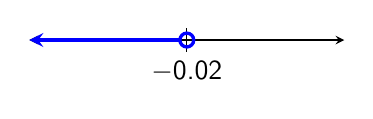
\begin{tikzpicture}
	\draw[<->] (-2,0) -- (2,0);
	\draw (0,0.15) -- (0,-0.15) node [below] {$-0.02$};
	\draw[->, very thick, blue, shorten <= 2.5pt] (0,0) -- (-2,0);
	\draw[blue, very thick] (0,0) circle [radius = 2.5pt];
	\end{tikzpicture}
\end{enumerate}
\end{multicols}
\chapter{Compound Inequalities}

Solve each. Graph your answers on a number line. 

\begin{multicols}{3}
\begin{enumerate}
	\item $-3 < x-8 \leq 12$
	\item $7 \leq 2x - 5 < 18$
	\item $x + 8 < 10 \text{ or } 5x - 9 \geq 26$
\end{enumerate}	\setcounter{Review}{\value{enumi}}
\end{multicols}
\begin{multicols}{3}
\begin{enumerate}	\setcounter{enumi}{\value{Review}}
	\item $x - 1.5 > 8 \text{ or } -x + 2 > 9$
	\item $4 \leq x + 7 < 9$
	\item $-2 < 6x + 10 \leq 5$
\end{enumerate}	\setcounter{Review}{\value{enumi}}
\end{multicols}
\begin{multicols}{3}
\begin{enumerate}	\setcounter{enumi}{\value{Review}}
	\item $3x > 9 \text{ or } -5x > 25$
	\item $8x+12 \leq 20   \text{ or } x + 12 > 9$
	\item $-8 \leq 3x+7 < 40$
\end{enumerate}	\setcounter{Review}{\value{enumi}}
\end{multicols}
\begin{multicols}{3}
\begin{enumerate}	\setcounter{enumi}{\value{Review}}
	\item $-5x + 9 \geq 12 \text{ or } 2x+6 > 5$
	\item $3x - 1 < x + 5 \text{ or } -x \geq 5+7x$
\end{enumerate}	\setcounter{Review}{\value{enumi}}
\end{multicols}



\newpage

\section{Answer Key}

\begin{multicols}{3}
\begin{enumerate}	
	\item $5 < x \leq 20$
	\item $6 \leq x < \frac{23}{2}$
	\item $x < 2 \text{ or } x \geq 7$
\end{enumerate}	\setcounter{Review}{\value{enumi}}
\end{multicols}
\begin{multicols}{3}
\begin{enumerate}	\setcounter{enumi}{\value{Review}}
	\item $x < -7 \text{ or } x > \frac{19}{2}$
	\item $-3 \leq x < 2$
	\item $-2 < x \leq -\frac{5}{6}$
\end{enumerate}	\setcounter{Review}{\value{enumi}}
\end{multicols}
\begin{multicols}{3}
\begin{enumerate}	\setcounter{enumi}{\value{Review}}
	\item $x < -5 \text{ or } x > 3$
	\item $\mathbb{R}$
	\item $-5 \leq x < 11$  \newline\\
    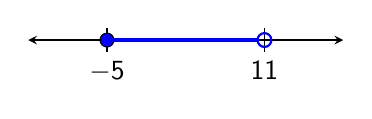
\begin{tikzpicture}
    \draw[<->] (-2,0) -- (2,0);
    \draw (-1,0.15) -- (-1,-0.15) node [below] {$-5$};
    \draw (1,0.15) -- (1,-0.15) node [below] {$11$};
    \draw [very thick, blue, shorten >=2.5pt, shorten >=2.5pt] (-1,0) -- (1,0);
    \draw [fill=blue] (-1,0) circle [radius = 2.5pt];
    \draw [thick, blue] (1,0) circle [radius = 2.5pt];
    \end{tikzpicture}
\end{enumerate}	\setcounter{Review}{\value{enumi}}
\end{multicols}
\begin{multicols}{3}
\begin{enumerate}	\setcounter{enumi}{\value{Review}}
	\item $x \leq -\frac{3}{5}$ or $x > -\frac{1}{2}$   \newline\\
    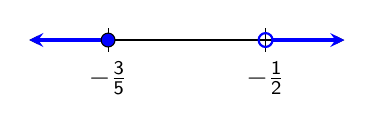
\begin{tikzpicture}
    \draw[<->] (-2,0) -- (2,0);
    \draw (-1,0.15) -- (-1,-0.15) node [below] {$-\frac{3}{5}$};
    \draw (1,0.15) -- (1,-0.15) node [below] {$-\frac{1}{2}$};
    \draw [->, very thick, blue, shorten <= 2.5pt] (-1,0) -- (-2,0);
    \draw [->, very thick, blue, shorten <= 2.5pt] (1,0) -- (2,0);
    \draw [fill=blue] (-1,0) circle [radius = 2.5pt];
    \draw [thick, blue] (1,0) circle [radius = 2.5pt];
    \end{tikzpicture}
    
    \item \item $x < 3$   \newline\\
    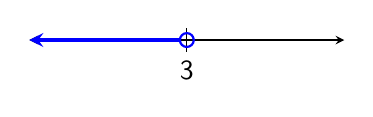
\begin{tikzpicture}
    \draw[<->] (-2,0) -- (2,0);
    \draw (0,0.15) -- (0,-0.15) node [below] {$3$};
    \draw [->, very thick, blue, shorten <= 2.5pt] (0,0) -- (-2,0);
    \draw [thick, blue] (0,0) circle [radius=2.5pt];
    \end{tikzpicture}
\end{enumerate}	\setcounter{Review}{\value{enumi}}
\end{multicols}



\chapter{Absolute Value Equations and Inequalities}

\section{Absolute Value Equations}

Solve each of the following.

\begin{multicols}{3}
\begin{enumerate}
	\item $|2x| = 10$
	\item $|3x-7|=8$
	\item $|5x+1| = -4$
\end{enumerate}	\setcounter{Review}{\value{enumi}}
\end{multicols}
\begin{multicols}{3}
\begin{enumerate}	\setcounter{enumi}{\value{Review}}
	\item $|x + 7| = 9$
	\item $|8x+16| = -24$
	\item $|-x-4| = -3$
\end{enumerate}	\setcounter{Review}{\value{enumi}}
\end{multicols}
\begin{multicols}{3}
\begin{enumerate}	\setcounter{enumi}{\value{Review}}
	\item $\left|\frac{1}{2}x + 2\right| = x - 3$
\end{enumerate}	\setcounter{Review}{\value{enumi}}
\end{multicols}



\section{Absolute Value Inequaltiies}

Solve each. Graph your answers on a number line.

\begin{multicols}{3}
\begin{enumerate}
	\item $|x-9| < 10$
	\item $|-x+1| \geq 7$
	\item $|x+8| < -1$
\end{enumerate}	\setcounter{Review}{\value{enumi}}
\end{multicols}
\begin{multicols}{3}
\begin{enumerate}	\setcounter{enumi}{\value{Review}}
	\item $|6x - 18| < 42$
	\item $|-2x+1| \geq 9$
	\item $|5x + 2| < 3x$
\end{enumerate}	\setcounter{Review}{\value{enumi}}
\end{multicols}
\begin{multicols}{3}
\begin{enumerate}	\setcounter{enumi}{\value{Review}}
	\item $|3x + 2| > 1$
    \item $|2x - 1| \leq 7$ 
    \item $|2x-8| \leq 3x$
\end{enumerate}	\setcounter{Review}{\value{enumi}}
\end{multicols}
\begin{multicols}{3}
\begin{enumerate}	\setcounter{enumi}{\value{Review}}
	\item $3\left| \frac{1}{3}x+9\right| > 27$
	\item $|0.1x+5.4| < 4.7$
	\item $|2x-5| \leq 12$
\end{enumerate}	\setcounter{Review}{\value{enumi}}
\end{multicols}
\begin{multicols}{3}
\begin{enumerate}	\setcounter{enumi}{\value{Review}}
	\item $|3x+1| > -2x+2$
	\item $-5|x+7| < -15$
\end{enumerate}	\setcounter{Review}{\value{enumi}}
\end{multicols}

\newpage

\section{Answer Key}

\subsection*{Absolute Value Equations}

\begin{multicols}{3}
\begin{enumerate}
	\item $x = \pm 5$
	\item $x = -\frac{1}{3} \text{ or } x = 5$
	\item $\emptyset$
\end{enumerate}	\setcounter{Review}{\value{enumi}}
\end{multicols}
\begin{multicols}{3}
\begin{enumerate}	\setcounter{enumi}{\value{Review}}
	\item $x = 2$ or $x = -16$
	\item $\emptyset$
	\item $\emptyset$
\end{enumerate}	\setcounter{Review}{\value{enumi}}
\end{multicols}
\begin{multicols}{3}
\begin{enumerate}	\setcounter{enumi}{\value{Review}}
	\item $x = 10$
\end{enumerate}	\setcounter{Review}{\value{enumi}}
\end{multicols}



\subsection*{Absolute Value Inequalities}

\begin{multicols}{3}
\begin{enumerate}
	\item $-1 < x < 19$ \newline\\
	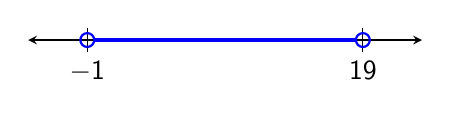
\begin{tikzpicture}
	\draw[<->] (-2.5,0) -- (2.5,0);
	\draw (-1.75,0.15) -- (-1.75,-0.15) node [below] {$-1$};
	\draw (1.75,0.15) -- (1.75,-0.15) node [below] {$19$};
	\draw[very thick, blue, shorten >= 2.5pt, shorten <= 2.5pt] (-1.75,0) -- (1.75,0);
	\draw[blue, thick] (-1.75,0) circle [radius=2.5pt];
	\draw[blue, thick] (1.75,0) circle [radius=2.5pt];
	\end{tikzpicture}
	\item $x \leq -6 \text{ or } x \geq 8$ \newline\\
	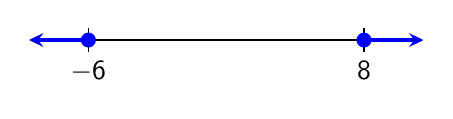
\begin{tikzpicture}
	\draw[<->] (-2.5,0) -- (2.5,0);
	\draw (-1.75,0.15) -- (-1.75,-0.15) node [below] {$-6$};
	\draw (1.75,0.15) -- (1.75,-0.15) node [below] {$8$};
	\draw[very thick, blue, ->] (-1.75,0) -- (-2.5,0);
	\draw[very thick, blue, ->] (1.75,0) -- (2.5,0);
	\draw[blue, fill=blue] (-1.75,0) circle [radius=2.5pt];
	\draw[blue, fill=blue] (1.75,0) circle [radius=2.5pt];
	\end{tikzpicture}
	\item $\emptyset$ \newline\\
	\begin{tikzpicture}
	\draw[<->] (-2.5,0) -- (2.5,0);
	\end{tikzpicture}
\end{enumerate}	\setcounter{Review}{\value{enumi}}
\end{multicols}
\begin{multicols}{3}
\begin{enumerate}	\setcounter{enumi}{\value{Review}}
	\item $-4 < x < 10$ \newline\\
    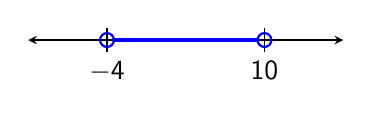
\begin{tikzpicture}
    \draw[<->] (-2,0) -- (2,0);
    \draw (-1,0.15) -- (-1,-0.15) node [below] {$-4$};
    \draw (1,0.15) -- (1,-0.15) node [below] {$10$};
    \draw [very thick, blue, shorten >= 2.5pt, shorten <= 2.5pt] (-1,0) -- (1,0);
    \draw [thick, blue] (-1,0) circle [radius = 2.5pt];
    \draw [thick, blue] (1,0) circle [radius = 2.5pt];
    \end{tikzpicture}  
    \item $x \leq -4$ or $x \geq 5$ \newline\\
    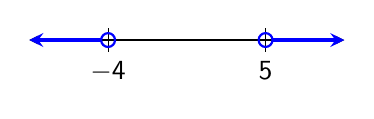
\begin{tikzpicture}
    \draw[<->] (-2,0) -- (2,0);
    \draw (-1,0.15) -- (-1,-0.15) node [below] {$-4$};
    \draw (1,0.15) -- (1,-0.15) node [below] {$5$};
    \draw [->, very thick, blue, shorten <= 2.5pt] (-1,0) -- (-2,0);
    \draw [->, very thick, blue, shorten <= 2.5pt] (1,0) -- (2,0);
    \draw [thick, blue] (-1,0) circle [radius = 2.5pt];
    \draw [thick, blue] (1,0) circle [radius = 2.5pt];
    \end{tikzpicture}
    \item $\emptyset$	\newline\\
    \begin{tikzpicture}
	\draw[<->] (-2.5,0) -- (2.5,0);
	\end{tikzpicture}
\end{enumerate}	\setcounter{Review}{\value{enumi}}
\end{multicols}
\begin{multicols}{3}
\begin{enumerate}	\setcounter{enumi}{\value{Review}}
	\item $x < -1$ or $x > \frac{1}{3}$ \newline\\
    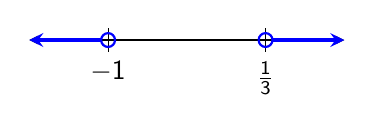
\begin{tikzpicture}
    \draw[<->] (-2,0) -- (2,0);
    \draw (-1,0.15) -- (-1,-0.15) node [below] {$-1$};
    \draw (1,0.15) -- (1,-0.15) node [below] {$\frac{1}{3}$};
    \draw[blue, very thick, ->, shorten <= 2.5pt] (-1,0) -- (-2,0);
    \draw[blue, very thick, ->, shorten <= 2.5pt] (1,0) -- (2,0);
    \draw[thick, blue] (-1,0) circle [radius=2.5pt];
    \draw[thick, blue] (1,0) circle [radius=2.5pt];
    \end{tikzpicture}
    \item $-3 \leq x \leq 4$ \newline\\
    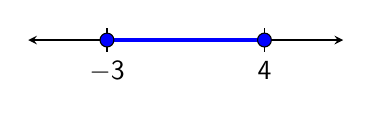
\begin{tikzpicture}
    \draw[<->] (-2,0) -- (2,0);
    \draw (-1,0.15) -- (-1,-0.15) node [below] {$-3$};
    \draw (1,0.15) -- (1,-0.15) node [below] {$4$};
    \draw[blue, very thick] (-1,0) -- (1,0);
    \draw[fill=blue] (-1,0) circle [radius=2.5pt];
    \draw[fill=blue] (1,0) circle [radius=2.5pt];
    \end{tikzpicture}
    \item $x \geq 1.6$ \newline\\
    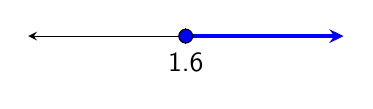
\begin{tikzpicture}
    \draw[<->] (-2,0) -- (2,0);
    \draw (0,0.1) -- (0,-0.1) node [below] {$1.6$};
    \draw[->, blue, very thick] (0,0) -- (2,0);
    \draw[fill=blue] (0,0) circle [radius=2.5pt];
    \end{tikzpicture}
\end{enumerate}	\setcounter{Review}{\value{enumi}}
\end{multicols}
\begin{multicols}{3}
\begin{enumerate}	\setcounter{enumi}{\value{Review}}
	\item $x < -54$ or $x > 0$ \newline\\
    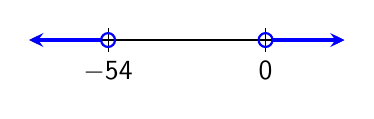
\begin{tikzpicture}
    \draw[<->] (-2,0) -- (2,0);
    \draw (-1,0.15) -- (-1,-0.15) node [below] {$-54$};
    \draw (1,0.15) -- (1,-0.15) node [below] {$0$};
    \draw[->, blue, very thick, shorten <= 2.5pt] (-1,0) -- (-2,0);
    \draw[->, blue, very thick, shorten <= 2.5pt] (1,0) -- (2,0);
    \draw[thick, blue] (-1,0) circle [radius=2.5pt];
    \draw[thick, blue] (1,0) circle [radius=2.5pt];
    \end{tikzpicture}
    \item $-101 < x < -7$ \newline\\
    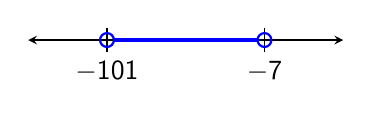
\begin{tikzpicture}
    \draw[<->] (-2,0) -- (2,0);
    \draw (-1,0.15) -- (-1,-0.15) node [below] {$-101$};
    \draw (1,0.15) -- (1,-0.15) node [below] {$-7$};
    \draw[blue, very thick, shorten <= 2.5pt, shorten >= 2.5pt] (-1,0) -- (1,0);
    \draw[thick, blue] (-1,0) circle [radius=2.5pt];
    \draw[thick, blue] (1,0) circle [radius=2.5pt];
    \end{tikzpicture} 
    \item $-3.5 \leq x \leq 8.5$ \newline\\
    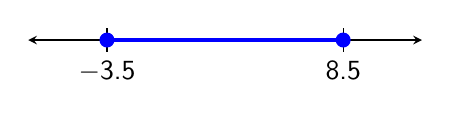
\begin{tikzpicture}
    \draw[<->] (-2.5,0) -- (2.5,0);
    \draw (-1.5,0.15) -- (-1.5,-0.15) node [below] {$-3.5$};
    \draw (1.5,0.15) -- (1.5,-0.15) node [below] {$8.5$};
    \draw[very thick, blue] (-1.5,0) -- (1.5,0);
    \draw[color=blue,fill=blue] (-1.5,0) circle [radius=2.5pt];
    \draw[color=blue,fill=blue] (1.5,0) circle [radius=2.5pt];
    \end{tikzpicture} 
\end{enumerate}	\setcounter{Review}{\value{enumi}}
\end{multicols}
\begin{multicols}{3}
\begin{enumerate}		\setcounter{enumi}{\value{Review}}
	\item $x < -3$ or $x > \frac{1}{5}$ \newline\\
    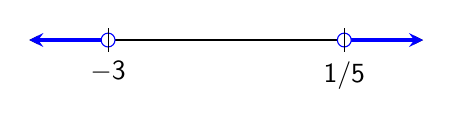
\begin{tikzpicture}
    \draw[<->] (-2.5,0) -- (2.5,0);
    \draw[very thick, blue,->] (-1.5,0) -- (-2.5,0);
    \draw[very thick, blue,->] (1.5,0) -- (2.5,0);
    \draw[color=blue,fill=white] (-1.5,0) circle [radius=2.5pt];
    \draw[color=blue,fill=white] (1.5,0) circle [radius=2.5pt];
    \draw (-1.5,0.15) -- (-1.5,-0.15) node [below] {$-3$};
    \draw (1.5,0.15) -- (1.5,-0.15) node [below] {$1/5$};
    \end{tikzpicture}
    \item $x < -10$ or $x > -4$ \newline\\
    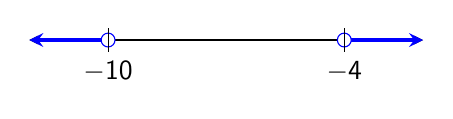
\begin{tikzpicture}
    \draw[<->] (-2.5,0) -- (2.5,0);
    \draw[very thick, blue,->] (-1.5,0) -- (-2.5,0);
    \draw[very thick, blue,->] (1.5,0) -- (2.5,0);
    \draw[color=blue,fill=white] (-1.5,0) circle [radius=2.5pt];
    \draw[color=blue,fill=white] (1.5,0) circle [radius=2.5pt];
    \draw (-1.5,0.15) -- (-1.5,-0.15) node [below] {$-10$};
    \draw (1.5,0.15) -- (1.5,-0.15) node [below] {$-4$};
    \end{tikzpicture}
\end{enumerate}		\setcounter{Review}{\value{enumi}}
\end{multicols}



\chapter{Factoring Techniques}

Factor each completely.

\begin{multicols}{4}
\begin{enumerate}
	\item $x^2 + 2x - 15$
	\item $a^2-15a+56$
	\item $8x^2+10x+3$
	\item $w^2+w-12$
\end{enumerate}	\setcounter{Review}{\value{enumi}}
\end{multicols}
\begin{multicols}{4}
\begin{enumerate}	\setcounter{enumi}{\value{Review}}
	\item $5b^2-9b-2$
	\item $12x^2+40x-7$
	\item $4x^2-4x-24$
    \item $18t^2-9t-5$
\end{enumerate}	\setcounter{Review}{\value{enumi}}
\end{multicols}
\begin{multicols}{4}
\begin{enumerate}	\setcounter{enumi}{\value{Review}}
	\item $6a^2 + 23a + 21$
	\item $x^2-12x+36$
    \item $9x^2-1$
    \item $4x^2+4x+1$
\end{enumerate}	\setcounter{Review}{\value{enumi}}
\end{multicols}
\begin{multicols}{4}
\begin{enumerate}	\setcounter{enumi}{\value{Review}}
	\item $x^3-x^2-2x$
	\item $6x^2-32x+10$
	\item $2x^3-9x^2-51x-40$
	\item $2x^3+3x^2-3x-2$
\end{enumerate}	\setcounter{Review}{\value{enumi}}
\end{multicols}
\begin{multicols}{4}
\begin{enumerate}	\setcounter{enumi}{\value{Review}}
	\item $4x^3+3x^2-42x+40$
	\item $6x^3-27x^2-168x$
\end{enumerate}	\setcounter{Review}{\value{enumi}}
\end{multicols}

The graph of a factorable expression is shown below. If the expression is in lowest terms (i.e. there is no number in front of all of the parentheses when it is factored) and contains integer coefficients, write the factored form of the expression.
\begin{multicols}{2}
\begin{enumerate}	\setcounter{enumi}{\value{Review}}
\item \mbox{} \newline\\
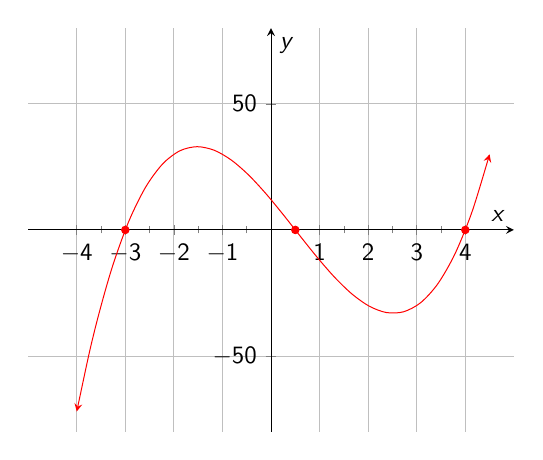
\begin{tikzpicture}[scale=0.9]
\begin{axis}[
axis lines=center, xmin = -5, xmax = 5, ymin=-80, ymax=80,
xtick = {-4,-3,...,4}, minor x tick num = 1, grid=major,
xlabel = $x$, ylabel=$y$]
\addplot [<->, smooth, red, domain=-4:4.5] {2*x^3-3*x^2-23*x+12};
\addplot [red, mark=*, only marks, mark size = 1.5] coordinates {(-3,0) (0.5,0) (4,0)};
\end{axis}
\end{tikzpicture}
\item \mbox{} \newline\\
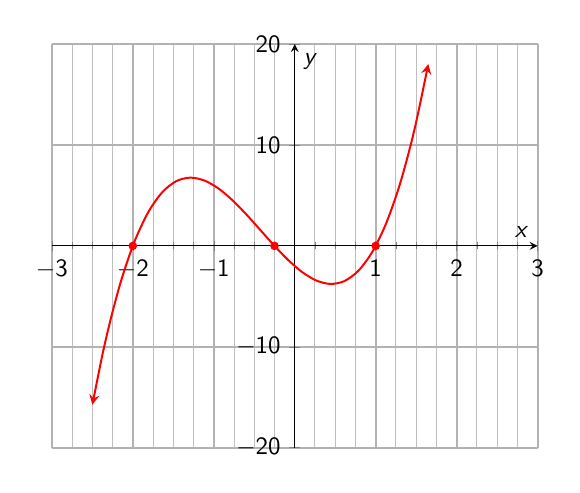
\begin{tikzpicture}[scale=0.9]
\begin{axis}[
axis lines=center, xmin = -3, xmax = 3, ymin=-20, ymax=20,
xtick = {-3,-2,...,3}, minor x tick num = 3, grid=both, major grid style={line width=.8pt,draw=gray!60},
xlabel = $x$, ylabel=$y$]
\addplot [<->, smooth, red, thick, domain=-2.5:1.65] {4*x^3 + 5*x^2 - 7*x - 2};
\addplot [red, mark=*, only marks, mark size = 1.5] coordinates {(-2,0) (-0.25,0) (1,0)};
\end{axis}
\end{tikzpicture}
\end{enumerate}	\setcounter{Review}{\value{enumi}}
\end{multicols}

\begin{multicols}{2}
\begin{enumerate}	\setcounter{enumi}{\value{Review}}
	\item \mbox{} \newline\\
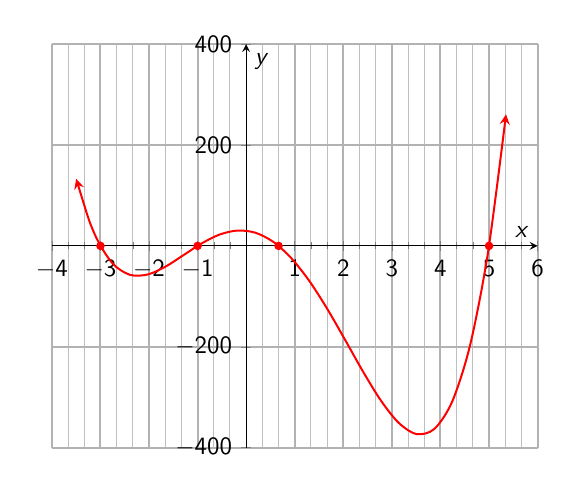
\begin{tikzpicture}[scale=0.9]
\begin{axis}[
axis lines=center, xmin = -4, xmax = 6, ymin=-400, ymax=400,
xtick = {-4,-3,...,6}, minor x tick num = 2, grid=both, major grid style={line width=.8pt,draw=gray!60},
xlabel = $x$, ylabel=$y$]
\addplot [<->, smooth, red, thick, domain=-3.5:5.35] {3*x^4 - 5*x^3 - 49*x^2 - 11*x + 30};
\addplot [red, mark=*, only marks, mark size = 1.5] coordinates {(-3,0) (-1,0) (2/3,0) (5,0)};
\end{axis}
\end{tikzpicture}
\item \mbox{} \newline\\

\end{enumerate}		\setcounter{Review}{\value{enumi}}
\end{multicols}


\newpage

\section{Answer Key}

\begin{enumerate}
	\item $(x+5)(x-3)$
    \item $(a-8)(a-7)$
    \item $(4x+3)(2x+1)$
    \item $(w+4)(w-3)$
	\item $(b-2)(5b+1)$
    \item $(2x+7)(6x-1)$
    \item $4(x-3)(x+2)$
    \item $(3t+1)(6t-5)$
    \item $(3a+7)(2a+3)$
    \item $(x-6)^2$
    \item $(3x-1)(3x+1)$
    \item $(2x+1)^2$
    \item $x(x-2)(x+1)$
    \item $2(3x-1)(x-5)$
    \item $(2x+5)(x+1)(x-8)$
    \item $(x+2)(2x+1)(x-1)$
    \item $(x+4)(4x-5)(x-2)$
    \item $3x(2x+7)(x-8)$
    
    \item $(x+3)(2x-1)(x-4)$
    \item $(x+2)(4x+1)(x-1)$
    \item $(x+3)(x+1)(x-1)(x-5)$
\end{enumerate}
\chapter{The Quadratic Formula}

Solve each. Exact answers only.

\begin{multicols}{3}
\begin{enumerate}
	\item $x^2-6x=-2$
	\item $4x^2 + 7x - 1 = 0$
    \item $8x^2 + 4x = 3$
\end{enumerate}	\setcounter{Review}{\value{enumi}}
\end{multicols}
\begin{multicols}{3}
\begin{enumerate}		\setcounter{enumi}{\value{Review}}
    \item $5x^2 + 6x - 2 = 3x^2 + 10$
    \item $7x^2-5 = 6x+11$
    \item $8x^2+2x+1=7x^2-8x-9$
\end{enumerate}	\setcounter{Review}{\value{enumi}}
\end{multicols}

\newpage

\section{Answer Key}

\begin{enumerate}
	\item $x = 3 \pm \sqrt{7}$
	\item $x = \frac{-7 \pm \sqrt{65}}{8}$
    \item $x = \frac{-1 \pm \sqrt{7}}{4}$
    \item $x = \frac{-3 \pm \sqrt{33}}{2}$
    \item $x = -\frac{8}{7}$, $x = 2$
    \item $x = -5 \pm \sqrt{15}$
\end{enumerate}
\chapter{Complex Numbers}

Simplify each.

\begin{multicols}{3}
\begin{enumerate}
	\item $(4-7i)+(-2+6i)$
	\item $(2-4i)-(2-3i)$
	\item $6 - (8 + 4i)$
\end{enumerate}	\setcounter{Review}{\value{enumi}}
\end{multicols}

\begin{multicols}{3}
\begin{enumerate}		\setcounter{enumi}{\value{Review}}
	\item $3(-2 + 7i)$
	\item $(2+3i)(-2-5i)$
	\item $(4+6i)(4-6i)$
\end{enumerate}	\setcounter{Review}{\value{enumi}}
\end{multicols}

\begin{multicols}{3}
\begin{enumerate}		\setcounter{enumi}{\value{Review}}
	\item $\frac{3+i}{2-i}$
	\item $3(7-4i)+2i(1+6i)$
	\item $(-2-6i)^2$
\end{enumerate}	\setcounter{Review}{\value{enumi}}
\end{multicols}

\begin{multicols}{3}
\begin{enumerate}		\setcounter{enumi}{\value{Review}}
	\item $\frac{2+3i}{4-5i}$
	\item $(2+3i)(-5+i)$
	\item $(-7 - 5i)^2$
\end{enumerate}	\setcounter{Review}{\value{enumi}}
\end{multicols}

\begin{multicols}{3}
\begin{enumerate}		\setcounter{enumi}{\value{Review}}
	\item $\frac{3+2i}{8+9i}$
	\item $\frac{-1+5i}{-9-2i}$
	\item $\left(\frac{2}{5} + \frac{1}{3}i\right)^2$
\end{enumerate}	\setcounter{Review}{\value{enumi}}
\end{multicols}


Solve each. Exact answers only.

\begin{multicols}{3}
\begin{enumerate}		\setcounter{enumi}{\value{Review}}
	\item $3x^2-7x+6=0$
	\item $5x^2-3x+2=0$
	\item $3x^2+7x-4=5x^2+2x+5$
\end{enumerate}	\setcounter{Review}{\value{enumi}}
\end{multicols}


\newpage

\section{Answer Key}

\begin{enumerate}
	\item $2-i$
    \item $-i$
    \item $-2-4i$
    \item $-6+21i$
    \item $11-16i$
    \item 52
    \item $1 + i$
    \item $9-10i$
    \item $-32+24i$
    \item $-\frac{7}{41}+\frac{22}{41}i$
    \item $-13-13i$
    \item $24+70i$
    \item $\frac{42}{145}-\frac{11}{145}i$
    \item $\frac{-1}{85}-\frac{47}{85}i$
    \item $\frac{11}{225} + \frac{4}{15}i$
    
    \item $x = \frac{7 \pm i\sqrt{23}}{6}$
    \item $x = \frac{3 \pm i \sqrt{31}}{10}$
    \item $x = \frac{5 \pm i\sqrt{47}}{4}$
\end{enumerate}
\chapter{Graphs of Quadratic Expressions}

Identify the vertex and axis of symmetry for each.

\begin{multicols}{3}
\begin{enumerate}   
    \item $y = 5x^2 - 15x + 7$
    \item $y = x^2 + 8x - 1$
    \item $y = \frac{1}{4}\left(x+3\right)^2 + 1$
\end{enumerate} \setcounter{Review}{\value{enumi}}
\end{multicols}

Write each of the following in general, $y = ax^2 + bx + c$, form.

\begin{multicols}{3}
\begin{enumerate}   \setcounter{enumi}{\value{Review}}
    \item $y = (x-7)^2 + 4$
	\item $y = -3(x+2)^2-5$
	\item $y = \frac{1}{4}(x-7)^2+1$
\end{enumerate} \setcounter{Review}{\value{enumi}}
\end{multicols}

\newpage


\section{Answer Key}

\begin{enumerate}
	\item Vertex: $\left(\frac{3}{2}, -\frac{17}{4}\right)$; \quad Axis of Symmetry: $x = \frac{3}{2}$
    \item Vertex: $(-4,-17)$; \quad Axis of Symmetry: $x = -4$
    \item Vertex: $(-3,1)$; \quad Axis of Symmetry: $x = -3$
    
    \item $y = x^2 - 14x + 53$
    \item $y = -3x^2-12x-17$
    \item $y = \frac{1}{4}x^2-\frac{7}{2}x+\frac{53}{4}$
\end{enumerate}
\appendix
\end{document}